\documentclass[
]{article}

\usepackage[utf8]{inputenc}

\providecommand{\tightlist}{%
  \setlength{\itemsep}{0pt}\setlength{\parskip}{0pt}}

\author{

}
\title{}

\Plainauthor{}

\Abstract{

}


%% publication information
%% \Volume{50}
%% \Issue{9}
%% \Month{June}
%% \Year{2012}
%% \Submitdate{}
%% \Acceptdate{2012-06-04}

\Address{
}


% Pandoc header



\begin{document}

\hypertarget{anuxe1lisis-de-la-tasa-de-interuxe9s}{%
\subsection{Análisis de la tasa de
interés}\label{anuxe1lisis-de-la-tasa-de-interuxe9s}}

Este reporte tiene la finalidad de visualizar los cambios en la tasa de
interés desde 2008 a 2020. Los \textbf{tipos de interés} son una de las
herramientas más importantes, utilizadas por los bancos centrales, para
llevar a cabo su política monetaría.

En México el objetivo de la política monetaria es mantener la
estabilidad de precios, es decir, controlar la inflación. Su
instrumentación la lleva a cabo el banco central en los mercados
financieros.

\hypertarget{visualizaciones}{%
\subsection{Visualizaciones}\label{visualizaciones}}

En las siguientes gráficas podemos ver cómo ha cambiado a lo largo de
los años la tasa de interés por el Banco de México.

\begin{CodeChunk}


\begin{center}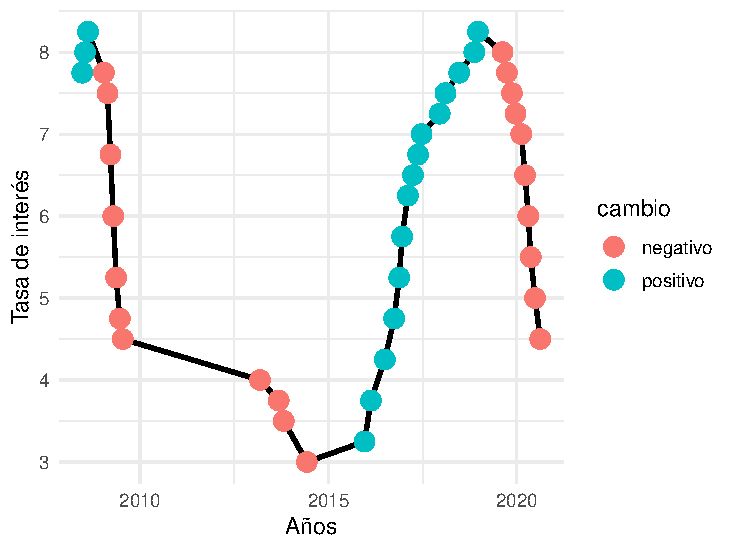
\includegraphics{reporte_tasa_files/figure-latex/graph1-1} \end{center}

\end{CodeChunk}

\begin{CodeChunk}


\begin{center}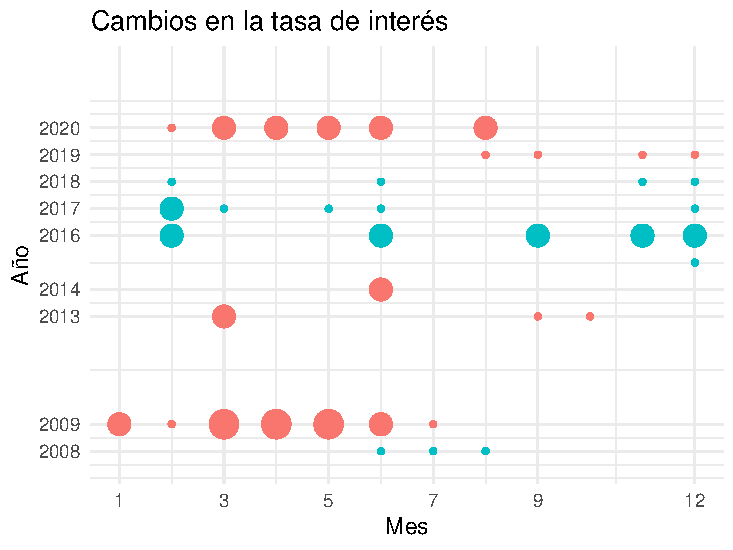
\includegraphics{reporte_tasa_files/figure-latex/graph2-1} \end{center}

\end{CodeChunk}



\end{document}
